% Inspired by Dan Spielman's template

\documentclass[10pt]{article}
\usepackage[T1]{fontenc}
\usepackage{amssymb}
\usepackage{amsmath}
\usepackage{graphicx}

\usepackage{tikz}
\usetikzlibrary{automata,positioning}
\usepackage{subfigure}
\usepackage{stackrel}
\usepackage{blindtext}

\oddsidemargin=0.15in
\evensidemargin=0.15in
\topmargin=-.5in
\textheight=9in
\textwidth=6.25in

\usepackage[colorlinks=true,breaklinks,pdfpagemode=none,linkcolor=blue, urlcolor = blue, citecolor=blue]{hyperref}
\usepackage{enumerate}

%\usepackage{enumitem}
%\setlist{itemsep=0mm}

%\usepackage[usenames,dvipsnames]{pstricks}
%\usepackage{epsfig}
\usepackage{amsmath,amsfonts,amssymb,bm}
%\usepackage{pst-grad} % For gradients
%\usepackage{pst-plot} % For axes

% Enviroment definitions (add your own here)

\newtheorem{theorem}{Theorem}
\newtheorem{corollary}[theorem]{Corollary}
\newtheorem{lemma}[theorem]{Lemma}
\newtheorem{observation}[theorem]{Observation}
\newtheorem{proposition}[theorem]{Proposition}
\newtheorem{definition}[theorem]{Definition}
\newtheorem{claim}[theorem]{Claim}
\newtheorem{fact}[theorem]{Fact}

\newenvironment{proof}{\noindent{\bf Proof}\hspace*{1em}}{\qed\bigskip}

% New commands (add your own here)

\newcommand{\eps}{\varepsilon}
\newcommand{\bbR}{\mathbb{R}}
\newcommand{\hv}{\hat{v}}
\newcommand{\hL}{\hat{L}}
\newcommand{\hlambda}{\hat{\lambda}}
\newcommand{\homega}{\hat{\omega}}
\newcommand{\hp}{\hat{p}}
\newcommand{\hW}{\hat{W}}
\newcommand{\cK}{\mathcal{K}}
\newcommand{\qed}{\rule{7pt}{7pt}}
\newcommand{\cF}{\mathcal{F}}

\begin{document}

    \noindent
    \begin{center}

        \hrulefill

        \vspace{5pt}

        \makebox[\textwidth]{ {\bf AB IdeaLab, Competitive Programming Team, Fall 18--Spring 19} \hfill  February 8, 2019}
        \vspace{0pt}

        {\Large \hfill  Lecture 3: FSA/Regular Expressions\hfill}
        \vspace{10pt}

        {\large \hfill  American Computer Science League, February Contest\hfill}
        \vspace{10pt}

        \makebox[\textwidth]{ {\it Primary Editor: Sanjit Bhat \hfill Secondary Editor: Alexander Sun} } % primary editor is the 'lecturer'

        \vspace{-3pt}
        \hrulefill
    \end{center}

\section{Fun Facts}
\begin{itemize}
\item Developed in 1951 by mathematician Stephen Cole Kleene.
\item Ken Thompson (one of the guys who developed UNIX) used regular expressions on an early Unix editor.
This eventually lead to its use in the famous UNIX tool grep.
\item Applications include string searching algorithms,  input verification, and search engines.
\item You can even use it inside your programming editor to find where you've put stuff.
\end{itemize}

\section{Background}
\paragraph{What are regular expressions?}
According to Wikipedia, regular expressions (regex) are ``a sequence of characters that define a search pattern.''
In other words, a regex defines a set of possible strings in a concise manner for
some later purpose.
For example, reali[sz]e defines the set \{realize, realise\} of possible strings.
This set can be later used for cross-referencing American-English spellings with
British-English spellings.

\paragraph{All the regex syntax you need to know.}
Regex includes \textit{metacharacters} that define more complex types
of string matching.
The following is a list of all the regex metacharacters you need to know:

\begin{enumerate}
\item \textbf{|, or, $\cup$}
These are booleans that tell the processor to take the set union of the regexes
on the left- and right-hand sides.
For instance, gr(a|e)y, gray or grey, and gr(a$\cup$e)y all define the set
\{gray, grey\}.

\item \textbf{$\lambda$}
The null or empty string.

\item \textbf{Quantification}
Defining the number of something allowed to occur.
Note that these all operate on a regex left of the operator.
    \begin{enumerate}
    \item \textbf{?}
    Zero or one.
    E.g., colou?r = \{color, colour\}.
    \item \textbf{*}
    Zero or more.
    This is also called the Kleene Star (named after the inventor, Stephen Kleene).
    \item \textbf{+}
    One or more.
    \end{enumerate}

\item \textbf{.}
Wildcard (a fill in for any character).
Combine . and * for a.*b, which accepts any string with a and b as the leftmost and rightmost
characters, respectively, with an arbitrary number of arbitrary characters inbetween.

\item \textbf{[\ldots]}
Set of possible character matches.
Think the reali[sz]e example above.
This can get slightly more complex by using hyphens to define ranges of possible characters.
E.g., [a-z] means every \textit{lowercase} char from a to z;
[abcx-z] means a, b, c, and x, y, z; and [a-cx-z] means a, b, c and x, y, z.

\item \textbf{[\string^\ldots]}
Set of characters not contained withing the brackets.
E.g., [\string^a-z] matches any character that is not a lowercase character from a to z.

\item \textbf{()}
Just like in math, parentheses imply grouping.
E.g., if we wanted the set \{gray, grey\}, gra|ey would give us \{gra, ey\}.
Instead, using parentheses we can get gr(a|e)y, which gives us the correct regex.
A more complex example is H(\"{a}|ae?)ndel, which matches \{Handel, H\"{a}ndel, Haendel\}.
\end{enumerate}

Order of operations: Kleene Star (*), concatenation (ab), and union($\cup$).
Because Kleene Star has the highest priority, a.*b accepts a string
with an arbitrary number of \textit{several different arbitrary} characters
 (e.g., \{acdb, \ldots\}), as opposed
to only an arbitrary number of a single arbitrary character (e.g., \{accb, \ldots\}).

\paragraph{Practicing the syntax via identity proofs.}
To make sure you understand the syntax and order of operations,
see if you can prove the following identities:
\begin{enumerate}
\item (a*)* = a*
\item aa* = a*a
\item aa* $\cup \lambda$ = a*
\item a(b $\cup$ c) = ab $\cup$ ac
\item a(ba)* = (ab)*a
\item (a $\cup$ b)* = (a* $\cup$ b*)*
\item (a $\cup$ b)* =(a*b*)*
\item (a $\cup$ b)* = a*(ba*)*
\end{enumerate}

\paragraph{How are regex interpreted by the computer?}
In a regex, there are two types of chars: literals and metacharacters.
Literals define regular characters, while metacharacters indicate
more nuanced behaviors.
After creating a regex, a regex processor transforms the characters into an internal
representation that can be thought of as a Finite State Automata (FSA).
FSAs are an abstract concept in theoretical computer science consisting of the following:
\begin{enumerate}
\item A finite number of states, of which exactly one is active at any given time
\item Transition rules to change the active state
\item An initial state
\item One or more final states
\end{enumerate}
We can draw an FSA by representing each state as a circle, the final state
as a double circle, the start state as the only state with an incoming arrow,
and the transition rules as labeled-edges connecting the states.
For instance, the following is an FSA diagram for the regex x+y+:

{\centering
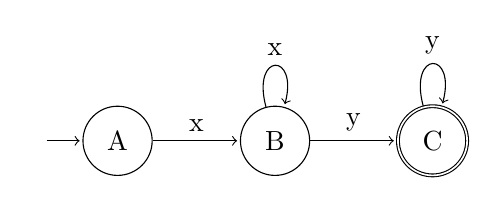
\begin{tikzpicture}[shorten >=1pt,node distance=2cm,on grid,auto]
   \node [state,initial, initial text=] (q_0) {A};
   \node [state, right of=q_0] (q_1) {B};
   \node [state, accepting, right of=q_1] (q_2) {C};
    \path[->]
    (q_0) edge node {x} (q_1)
    (q_1) edge node {y} (q_2)
          edge [loop above] node {x} ()
    (q_2) edge [loop above] node {y} ();
\end{tikzpicture}

}

If you would like to learn more about FSAs, I recommend the Wikipedia page.
Outside the ACSL bubble, automata and finiteness
are an important field of research in theoretical CS\@.
They connect back to problems such as P vs. NP and whether a program
will stop in a reasonable amount of time or even in an infinite amount of time.

\paragraph{Testing regex syntax.}
If you would like to practice regex and have your code actually
matched against strings, I recommend \href{https://regexr.com/}{this} website.

\section{Exercises}
\subsection{Translate an FSA to a Regular Expression}
\label{par:translate}
\begin{enumerate}
\item Find a simplified Regular Expression for the following FSA:

{\centering
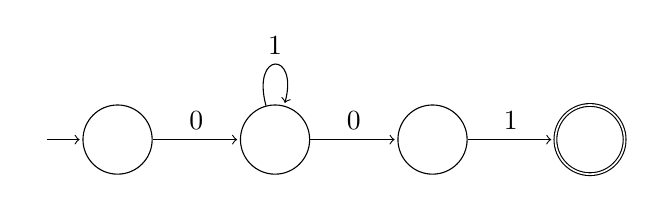
\begin{tikzpicture}[shorten >=1pt,node distance=2cm,on grid,auto]
   \node [state,initial,initial text=] (q_0) {};
   \node [state, right of=q_0] (q_1) {};
   \node [state, right of=q_1] (q_2) {};
   \node [state, accepting, right of=q_2] (q_3) {};
    \path[->]
    (q_0) edge node {0} (q_1)
    (q_1) edge node {0} (q_2)
          edge [loop above] node {1} ()
    (q_2) edge node {1} (q_3);
\end{tikzpicture}

}

\item Find a simplified Regular Expression for the following FSA:

{\centering
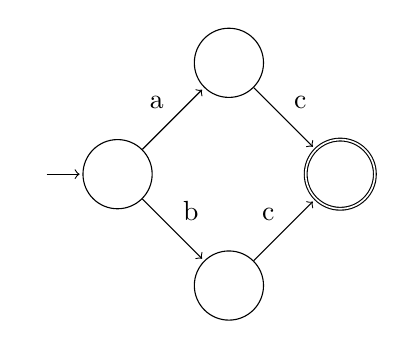
\begin{tikzpicture}[shorten >=1pt,node distance=2cm,on grid,auto]
   \node [state,initial,initial text=] (q_0) {};
   \node [state, above right=of q_0] (q_1) {};
   \node [state, below right=of q_0] (q_2) {};
   \node [state, accepting, below right=of q_1] (q_3) {};
    \path[->]
    (q_0) edge node {a} (q_1)
          edge node {b} (q_2)
    (q_1) edge node {c} (q_3)
    (q_2) edge node {c} (q_3);
\end{tikzpicture}

}

\item List all of the following FSAs which represent 1*01*0:

    \begin{enumerate}
    \item
    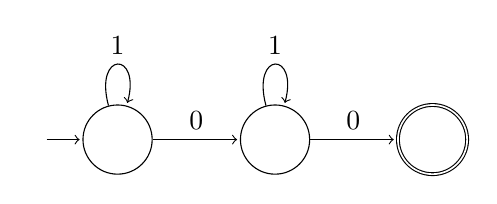
\begin{tikzpicture}[shorten >=1pt,node distance=2cm,on grid,auto]
       \node [state,initial,initial text=] (q_0) {};
       \node [state, right of=q_0] (q_1) {};
       \node [state, accepting, right of=q_1] (q_2) {};
        \path[->]
        (q_0) edge [loop above] node {1} ()
              edge node {0} (q_1)
        (q_1) edge [loop above] node {1} ()
              edge node {0} (q_2);
    \end{tikzpicture}

    \item
    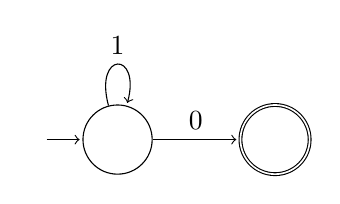
\begin{tikzpicture}[shorten >=1pt,node distance=2cm,on grid,auto]
       \node [state,initial,initial text=] (q_0) {};
       \node [state, accepting, right of=q_0] (q_1) {};
        \path[->]
        (q_0) edge [loop above] node {1} ()
              edge node {0} (q_1);
    \end{tikzpicture}

    \item
    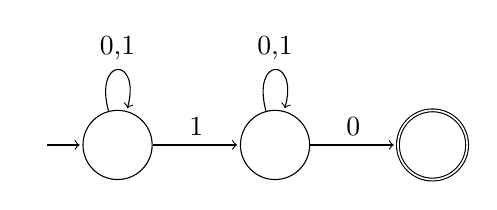
\begin{tikzpicture}[shorten >=1pt,node distance=2cm,on grid,auto]
       \node [state,initial,initial text=] (q_0) {};
       \node [state, right of=q_0] (q_1) {};
       \node [state, accepting, right of=q_1] (q_2) {};
        \path[->]
        (q_0) edge [loop above] node {0,1} ()
              edge node {1} (q_1)
        (q_1) edge [loop above] node {0,1} ()
              edge node {0} (q_2);
    \end{tikzpicture}

    \item
    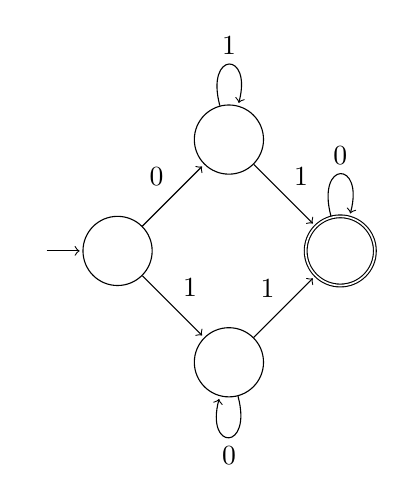
\begin{tikzpicture}[shorten >=1pt,node distance=2cm,on grid,auto]
       \node [state,initial,initial text=] (q_0) {};
       \node [state, above right=of q_0] (q_1) {};
       \node [state, below right=of q_0] (q_2) {};
       \node [state, accepting, below right=of q_1] (q_3) {};
        \path[->]
        (q_0) edge node {0} (q_1)
              edge node {1} (q_2)
        (q_1) edge [loop above] node {1} ()
              edge node {1} (q_3)
        (q_2) edge [loop below] node {0} ()
              edge node {1} (q_3)
        (q_3) edge [loop above] node {0} ();
    \end{tikzpicture}
    \end{enumerate}
\end{enumerate}

\subsection{Simplify a Regular Expression}
\label{par:simplify}

\subsection{Determine which Regular Expressions or FSAs are equivalent}
\label{par:equivalent}
\begin{enumerate}
\item Which, if any, of the following Regular Expressions are equivalent?
    \begin{enumerate}
    \item (a$\cup$b)(ab*)(b*$\cup$a)
    \item (aab*$\cup$bab*)a
    \item aab*$\cup$bab*$\cup$aaba$\cup$bab*a
    \item aab*$\cup$bab*$\cup$aab*a$\cup$bab*a
    \item a*$\cup$b*
    \end{enumerate}
\end{enumerate}

\subsection{Determine which strings are accepted by either an FSA or a Regular Expression}
\label{par:accepted}
\begin{enumerate}
\item Which of the following strings are accepted by the following Regular Expression     ``00*1*1U11*0*0''?
    \begin{enumerate}
    \item 0000001111111
    \item 1010101010
    \item 1111111
    \item 0110
    \item 10
    \end{enumerate}
\item Which of the following strings match the regular expression
pattern ``[A-D]*[a-d]*[0-9]''?
    \begin{enumerate}
    \item ABCD8
    \item abcd5
    \item ABcd9
    \item AbCd7
    \item X
    \item abCD7
    \item DCCBBBaaaa5
    \end{enumerate}
\item Which of the following strings match the regular expression
pattern ``Hi?g+h+[\string^a-ceiou]''?
    \begin{enumerate}
    \item Highb
    \item HiiighS
    \item HigghhhC
    \item Hih
    \item Hghe
    \item Highd
    \item HgggggghX
    \end{enumerate}
\end{enumerate}

%\newpage
\section{Solutions}

\subsection{Answers for Section~\ref{par:translate}}
\begin{enumerate}
\item 01*01
\item (a|b)c or ac $\cup$ bc
\item a. The other choices correspond to 1*0, (0$\cup$1)*1(0$\cup$1)*0, and 01*10*$\cup$10*10*
\end{enumerate}

\subsection{Answers for Section~\ref{par:equivalent}}
\begin{enumerate}
\item B is different from the rest because it requires an ending `a'.
E is different from the rest because it doesn't allow for alternating a's and b's.
C and D are different because of the third `or' condition.
Upon very close inspection, A and D are equivalent (check this carefully yourself).
Therefore, A and D are the answers.
\end{enumerate}

\subsection{Answers for Section~\ref{par:accepted}}
\begin{enumerate}
\item 0000001111111 and 10
\item ABCD8, abcd5, ABcd9, and DCCBBBaaaa5
\item HigghhhC, Highd, and HgggggghX
\end{enumerate}

%\begin{thebibliography}{9}
%    \bibitem{deep_learning}
%    Lecun, Y., Bengio, Y., and Hinton, G. (2015).
%    Deep learning.
%    Nature, 521(7553), 436-444.
%\end{thebibliography}
\end{document}